% To be \input{}'ed from the various subfolders - do not attempt to compile on
% its own!

\documentclass[10pt]{beamer}
\usepackage[T1]{fontenc}
\usepackage[utf8]{inputenc}

\graphicspath{{}{figures/}{screenshots/}}

\usetheme[progressbar=frametitle]{metropolis}
\usepackage{appendixnumberbeamer}

\usepackage{booktabs}
\usepackage[scale=2]{ccicons}

\usepackage{pgfplots}
\pgfplotsset{compat=1.12}
\usepgfplotslibrary{dateplot}

\usetikzlibrary{calc,fit,patterns}
\usepackage[absolute,overlay]{textpos}

\usepackage{xspace}
\newcommand{\themename}{\textbf{\textsc{metropolis}}\xspace}

\newcommand*{\file}[1]{\texttt{#1}}

\usepackage{xcolor}
\usepackage{listings}
\lstset{columns=fullflexible}
\lstdefinelanguage{EOL}{
morekeywords={delete,import,for,while,in,and,or,self,operation,return,def,var,throw,if,new,else,transaction,abort,
break,breakAll,continue,assert,assertError,not, switch, case, default},
sensitive=true,
morecomment=[l]{//},
morecomment=[l]{--},
morecomment=[s]{/*}{*/},
morecomment=[s]{-*}{*-},
morestring=[b]",
morestring=[b]',
showstringspaces=false
}

\lstnewenvironment{java}{\lstset{language=Java,
		frame=tb,
        tabsize=3,
        morekeywords={implies, in, result},
        basicstyle=\footnotesize,
        keywordstyle=\bfseries,
        ndkeywordstyle=\bfseries,
        commentstyle=\itshape,
		morecomment=[l]{--},
        stringstyle=\ttfamily,
		showspaces=false,
        flexiblecolumns,
        literate={->}{$\to$}{2} {--}{-$\,$-}{2} {<=}{$\le$}{2} {>=}{$\ge$}{2} {<>}{$<\,>$}{3},
        sensitive, extendedchars, texcl}}{}

\lstnewenvironment{ocl}{\lstset{language=[decorative]OCL,
	frame=tb,
	tabsize=3,
	morekeywords={implies,result,flatten,body,init,OrderedSet,Tuple,TupleType,def,attr,oclIsUndefined,oclIsInvalid,OclState,let,in},
	basicstyle=\footnotesize,
	keywordstyle=\bfseries,
	ndkeywordstyle=\bfseries,
	commentstyle=\itshape,
	stringstyle=\ttfamily,
	showspaces=false,
	flexiblecolumns,
	literate={->}{$\to$}{2} {--}{-$\,$-}{2} {<=}{$\le$}{2} {>=}{$\ge$}{2} {<>}{$<\,>$}{3},
	sensitive, extendedchars, texcl}}{}


\lstdefinelanguage{gremlin}{
morekeywords={as,def,fill,filter,groupCount,has,idx,inE,inV,is,label,length,match,outE,outV,v,values},
sensitive=true,
morecomment=[l]{//}
}

% "page cs" coordinate system
% From http://tex.stackexchange.com/questions/89588/
%
% Defining a new coordinate system for the page:
%
% --------------------------
% |(-1,1)    (0,1)    (1,1)|
% |                        |
% |(-1,0)    (0,0)    (1,0)|
% |                        |
% |(-1,-1)   (0,-1)  (1,-1)|
% --------------------------
\makeatletter
\def\parsecomma#1,#2\endparsecomma{\def\page@x{#1}\def\page@y{#2}}
\tikzdeclarecoordinatesystem{page}{
    \parsecomma#1\endparsecomma
    \pgfpointanchor{current page}{north east}
    % Save the upper right corner
    \pgf@xc=\pgf@x%
    \pgf@yc=\pgf@y%
    % save the lower left corner
    \pgfpointanchor{current page}{south west}
    \pgf@xb=\pgf@x%
    \pgf@yb=\pgf@y%
    % Transform to the correct placement
    \pgfmathparse{(\pgf@xc-\pgf@xb)/2.*\page@x+(\pgf@xc+\pgf@xb)/2.}
    \expandafter\pgf@x\expandafter=\pgfmathresult pt
    \pgfmathparse{(\pgf@yc-\pgf@yb)/2.*\page@y+(\pgf@yc+\pgf@yb)/2.}
    \expandafter\pgf@y\expandafter=\pgfmathresult pt
}
\makeatother
% Draws a grid for easier referencing of page cs values
\newcommand{\printtikzpagegrid}{
  \tiny
  \begin{tikzpicture}[overlay,remember picture,every node/.style={inner sep=.1em,draw=black!20,fill=white}]
    \foreach \x in {0,...,9} {
      \foreach \y in {0,...,9} {
        \node at (page cs:0.\x,0.\y) {};
        \node at (page cs:0.\x,-0.\y) {};
        \node at (page cs:-0.\x,0.\y) {};
        \node at (page cs:-0.\x,-0.\y) {};
      }
    }
    \node at (page cs:0,0) {0,0};
    \node at (page cs:0.5,0.5) {.5,.5};
    \node at (page cs:0.5,-0.5) {.5,-.5};
    \node at (page cs:-0.5,0.5) {-.5,.5};
    \node at (page cs:-0.5,-0.5) {-.5,-.5};
    \node at (page cs:1,1) {1,1};
    \node at (page cs:1,-1) {1,-1};
    \node at (page cs:-1,1) {-1,1};
    \node at (page cs:-1,-1) {-1,-1};
  \end{tikzpicture}
  \normalsize
}

\title{Taming Large Models\\with Hawk and NeoEMF}
%\subtitle{A modern beamer theme}
\date{MoDELS'2018, 14--19 October 2018}
\author{A. García-Domínguez, D. S. Kolovos, K. Barmpis, G. Daniel, G. Sunyé}
%\institute{Center for modern beamer themes}
% \titlegraphic{\hfill\includegraphics[height=1.5cm]{logo.pdf}}


\begin{document}

\maketitle

\pgfset{/metropolis/inner/sectionpage/.cd, none}
\section{Introduction}
\section{Hawk}

\pgfset{/metropolis/inner/sectionpage/.cd, progressbar}
\section{NeoEMF}

\begin{frame}[c]\frametitle{NeoEMF: overview}
	\begin{itemize}
	\item Handle large models with task-specific databases
	\item Lazy-loading
	\item Compliant with the EMF API
	\begin{itemize}
		\item Easy to integrate in existing applications
		\item EMF-Compatible code generation
	\end{itemize}
	\item Advanced caching (\& prefetching strategies)
	\item Efficient XMI importer
	\end{itemize}
\end{frame}

\begin{frame}[t]\frametitle{NeoEMF: Architecture}
  \begin{center}
    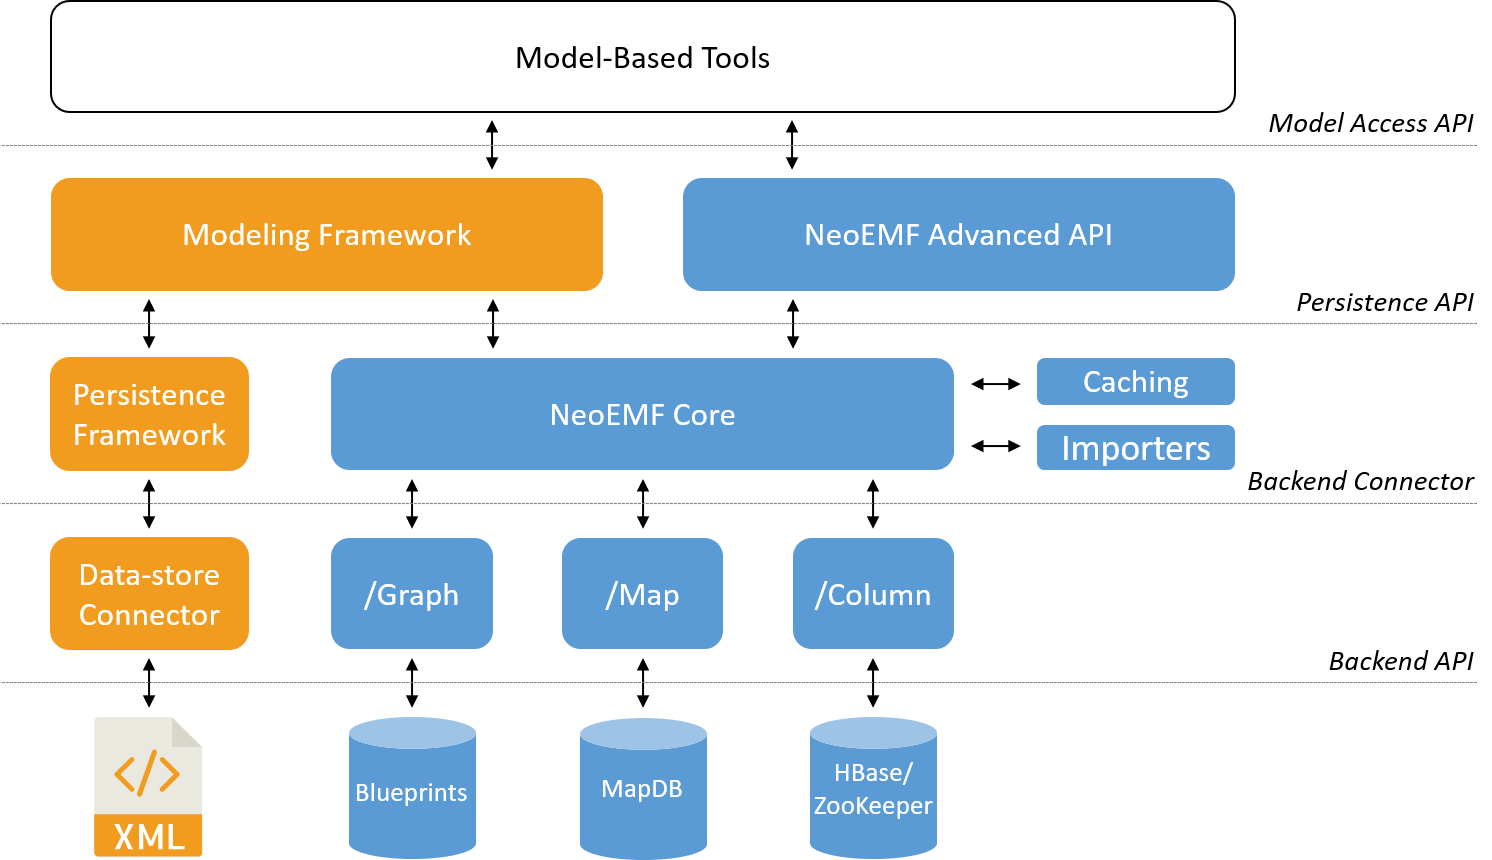
\includegraphics[width=\textwidth]{neoemf-architecture.png}
  \end{center}
\end{frame}

\begin{frame}[c]\frametitle{NeoEMF: datastores~\cite{DBLP:conf/models/DanielSBTVGC16}}
	\begin{itemize}
	\item \textbf{NeoEMF/Graph}
		\begin{itemize}
		\item Efficient model traversal using rich query language
		\item Mogwaï framework (OCL to Gremlin translation)
		\end{itemize}
	\item \textbf{NeoEMF/Map}
		\begin{itemize}
		\item Fast access to atomic operations
		\item Designed for EMF-API calls
		\end{itemize}
	\item \textbf{NeoEMF/Column}
		\begin{itemize}
		\item Transparent model distribution
		\item Concurrent read/write
		\item Distributed model transformations (ATL-MR)
		\end{itemize}
	\end{itemize}
\end{frame}

\begin{frame}[t]\frametitle{NeoEMF: project website}
  \begin{center}
    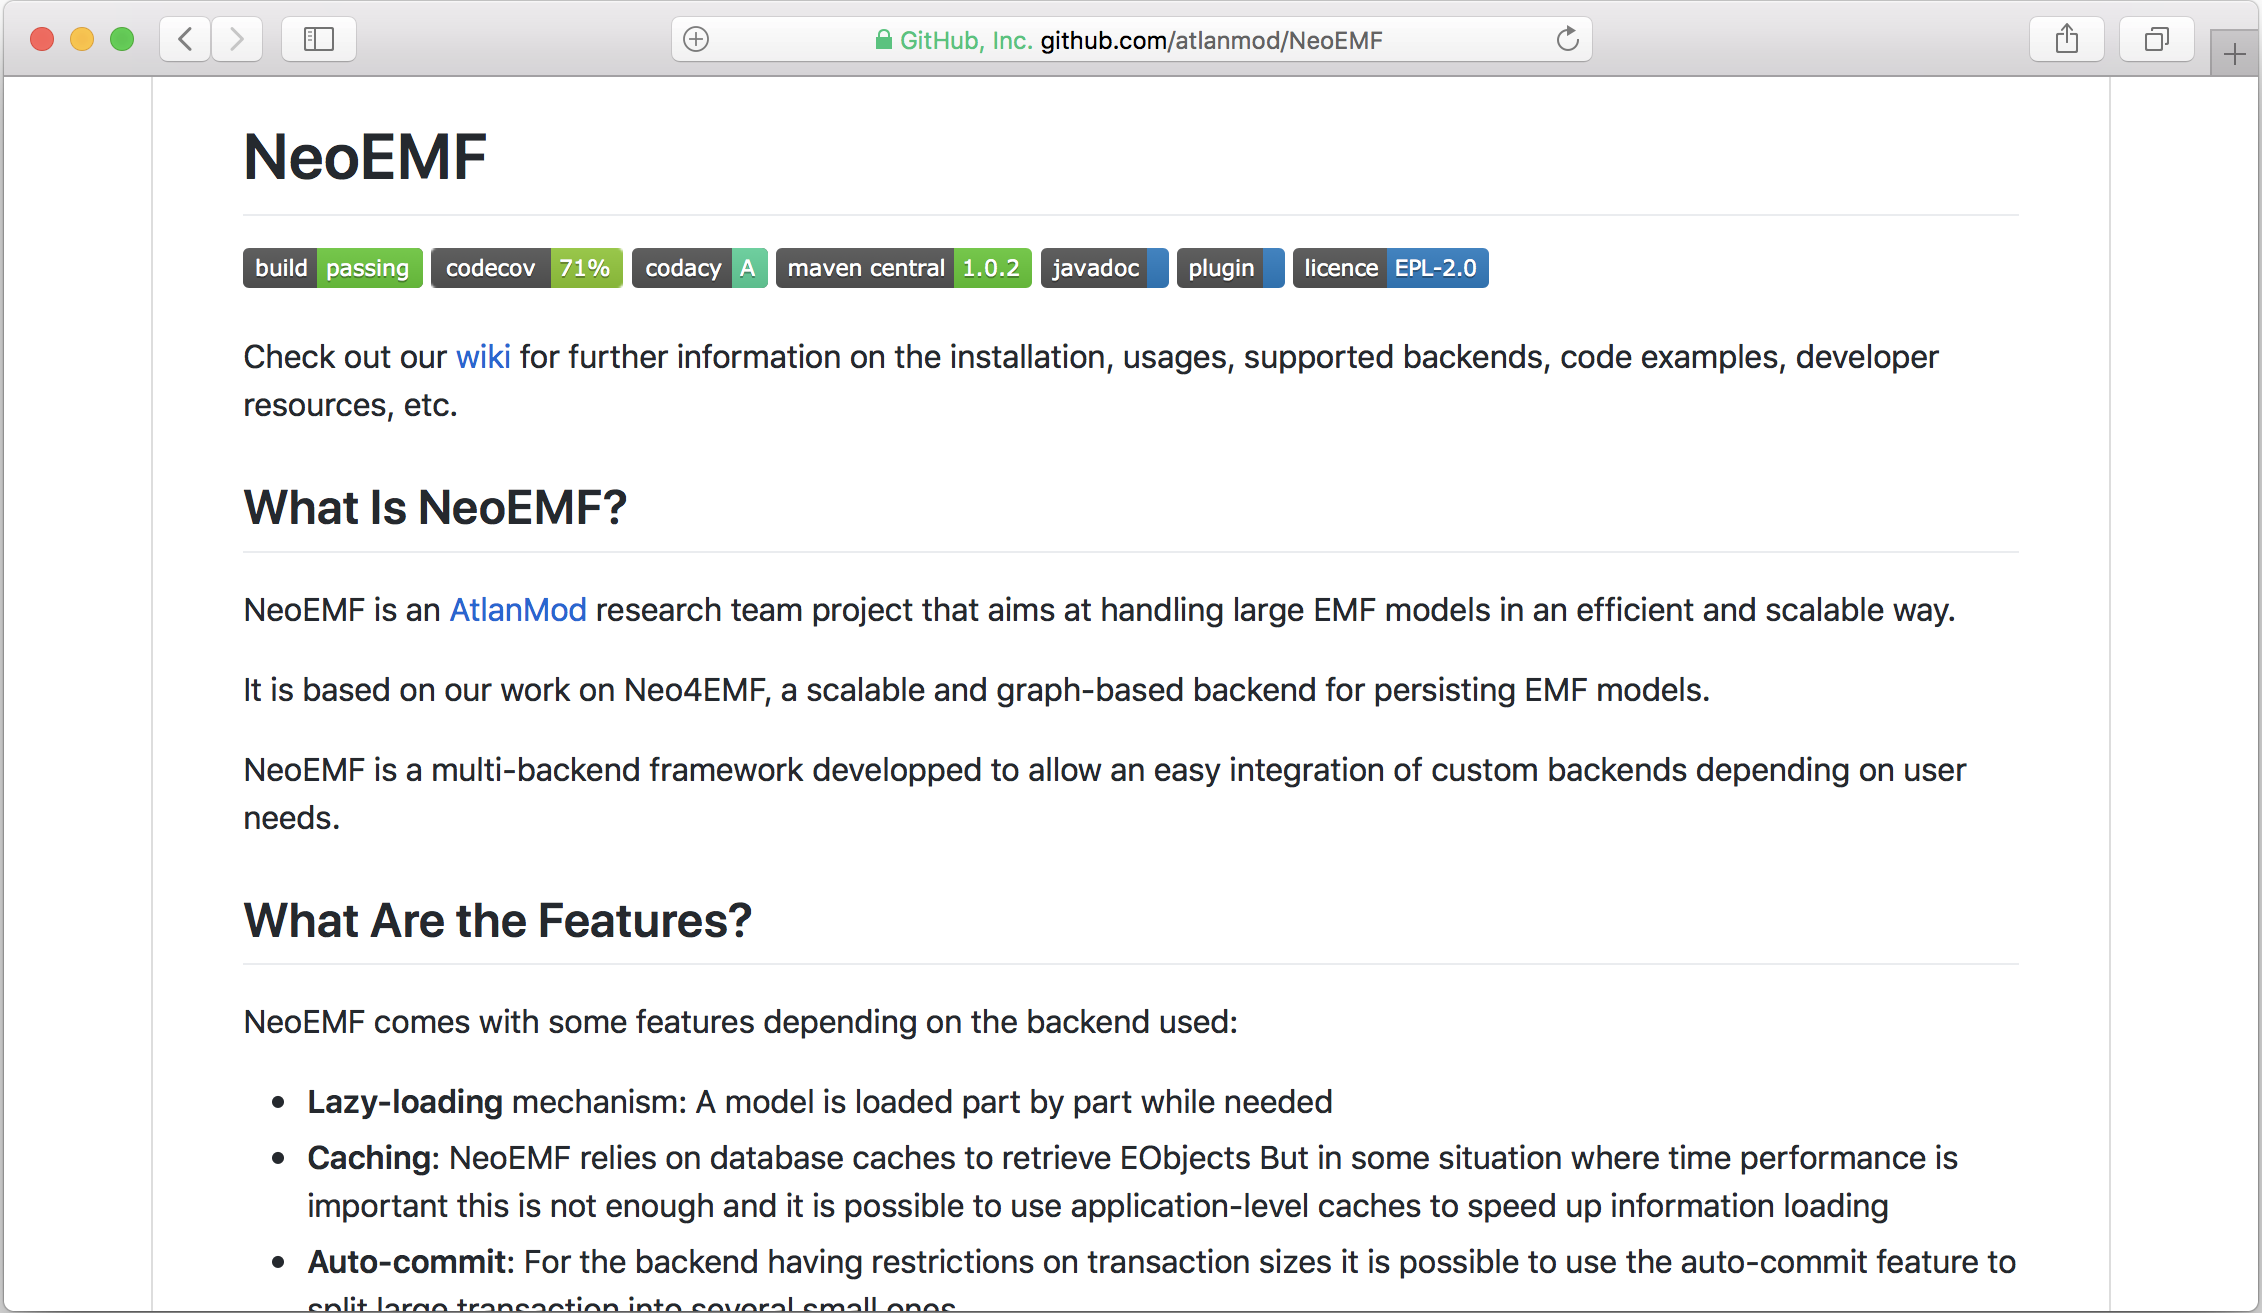
\includegraphics[width=\textwidth]{neoemf-github.png}
  \end{center}
	
  \begin{itemize}
  \item \url{https://github.com/atlanmod/NeoEMF}
  \item Open source project under the Eclipse Public License 2.0
  \end{itemize}
\end{frame}

\begin{frame}[fragile]\frametitle{NeoEMF: initialise a new resource}
	\begin{enumerate}
	\item Register the Persistence Backend Factory.
	\item Create a ResourceSet and register the PersistentResourceFactory
	\item Create a new URI to locate a file-based resource.
	\item Create the resource.
	\end{enumerate}
	
  \begin{java}
PersistenceBackendFactoryRegistry.register(
			BlueprintsURI.SCHEME,
			BlueprintsPersistenceBackendFactory.getInstance());  
  
ResourceSet resourceSet = new ResourceSetImpl();
resourceSet.getResourceFactoryRegistry().getProtocolToFactoryMap()
			.put(BlueprintsURI.SCHEME,
					PersistentResourceFactory.getInstance());
						
URI uri = BlueprintsURI.createFileURI(new File("<db_path>"));
						
Resource resource = resourceSet.createResource(uri);
    
// EMF resource stored in an in-memory Blueprints graph
  \end{java}
\end{frame}

\begin{frame}[fragile]\frametitle{NeoEMF: persist a resource}
	
	\begin{enumerate}
	\item Create a new option builder (backend-specific).
	\item Save the resource.
	\item Manipulate the resource by accessing the local database
	\end{enumerate}
  \begin{java}
Map<String, Object> options = BlueprintsNeo4jOptionsBuilder.newBuilder()
		.weakCache().autocommit().cacheSizes()

resource.save(options);
// Resource saved in a local Neo4j database
resource.getContents() 
// [...]
  \end{java}
	
\end{frame}

\begin{frame}[fragile]\frametitle{NeoEMF: modify an existing resource}
	\begin{enumerate}
	\item Load resource using the same option builder.
	\item Navigate its content and perform update operations
	\item Save the resource (automatically done with \emph{autocommit} option)
	\end{enumerate}
	
  \begin{java}
Map<String, Object> options = BlueprintsNeo4jOptionsBuilder.newBuilder()
		.weakCache().autocommit().cacheSizes()

URI uri = BlueprintsURI.createFileURI(new File("<db_path>"));

resourceSet.createResource(uri)
resource.load(options);

// Model manipulation operation (complete EMF API support)
MyClass myClass = (MyClass) resource.getContents().get(0);
myClass.setName("NewName");

// Save the modification in the local Neo4j database
resource.save(config.asMap());
  \end{java}
\end{frame}

\begin{frame}[standout]
  Demo time!

  Let's import a Java model, save it in Neo4j and MapDB, and query the database.
\end{frame}

\section{Mogwa\"i}

\begin{frame}[c]\frametitle{Mogwa\"i: motivation}
	\begin{itemize}
		\item NeoEMF improves model scalability, but ...
	\end{itemize}
  \begin{center}
    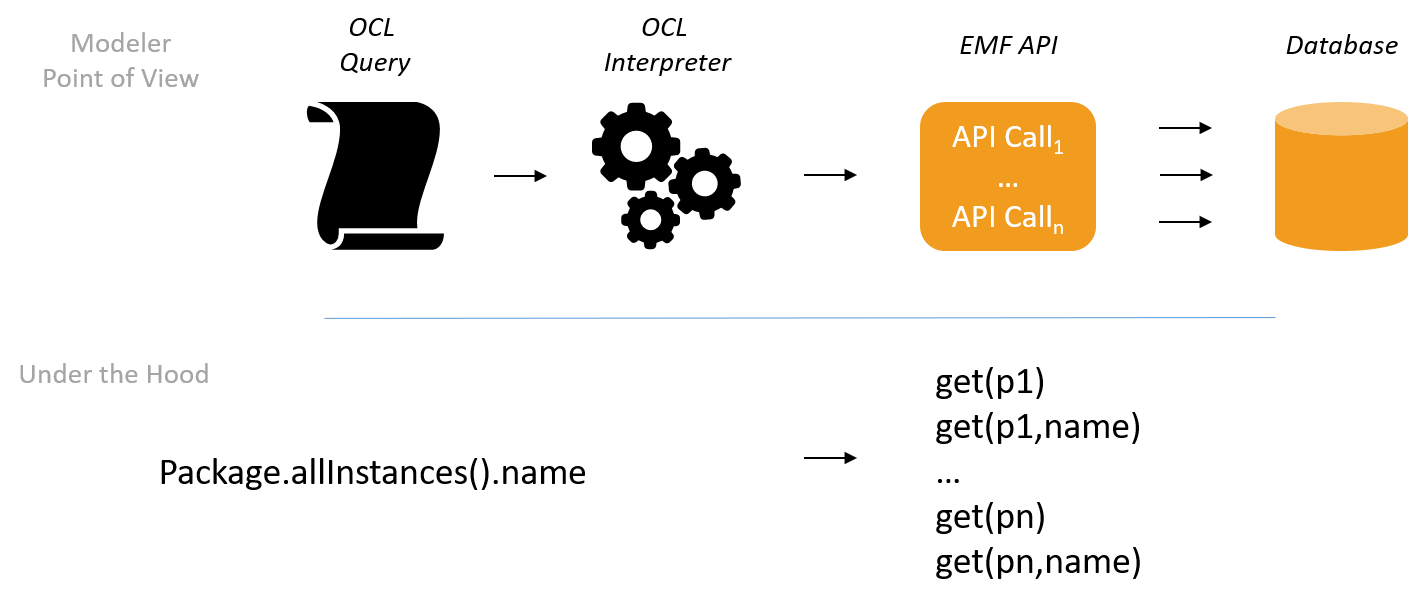
\includegraphics[width=\textwidth]{emf-ocl.png}
  \end{center}
\end{frame}

\begin{frame}[c]\frametitle{Mogwa\"i: motivation}
	\begin{itemize}
	\item Low-level model handling APIs
	\begin{itemize}
	\item Not aligned with the database capabilities
	\end{itemize}
	\item Fragmented queries on the database
	\begin{itemize}
	\item Not efficient
	\item Remote databases
	\end{itemize}
	\item Intermediate object reification
	\begin{itemize}
	\item Memory consumption
	\item Execution time overhead
	\end{itemize}	
	\end{itemize}
\end{frame}

\begin{frame}[c]\frametitle{Mogwa\"i: motivation}
\begin{itemize}
	\item Database queries are efficient but
	\begin{itemize}
		\item Modern persistence frameworks typically rely on NoSQL databases
		\begin{itemize}
		\item Multiple query languages
		\item Multiple data representations
		\item Low-level queries are hard to understand and maintain
		\item Modeling expertise vs. Database expertise
		\end{itemize}
	\end{itemize}
	\item Solution: generate them!
	\end{itemize}
\end{frame}

\begin{frame}[t]\frametitle{Mogwa\"i: architecture~\cite{DBLP:conf/rcis/DanielSC16}}
  \begin{center}
    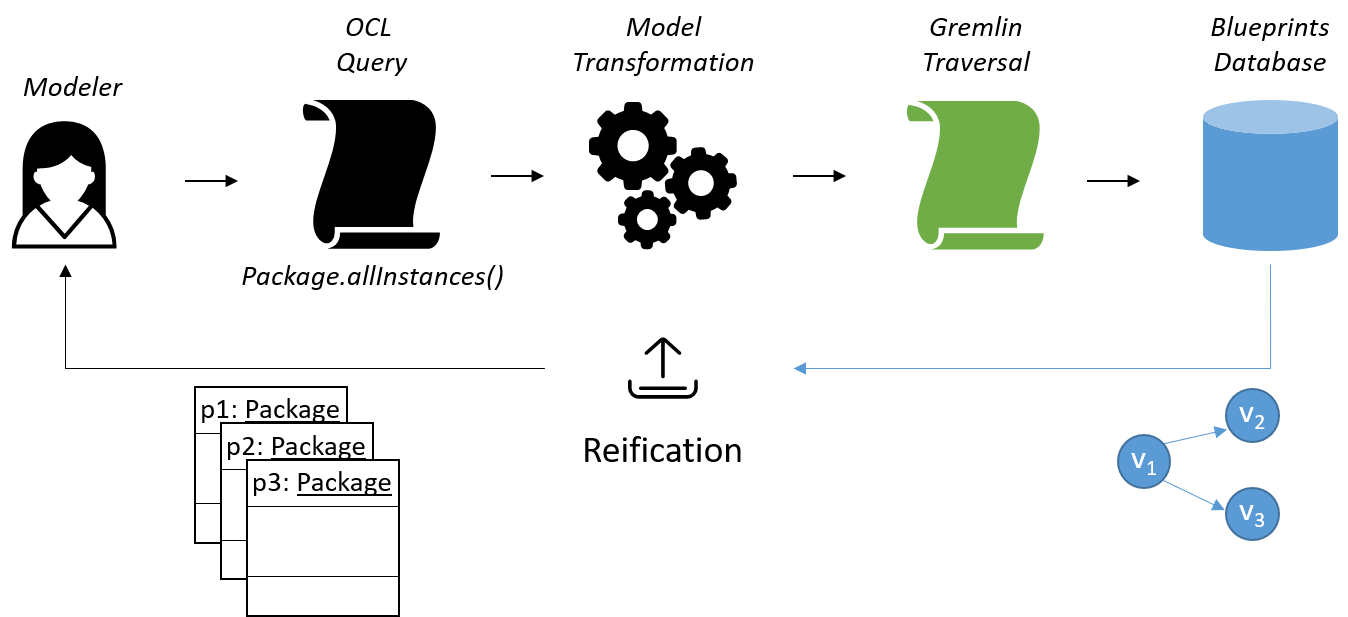
\includegraphics[width=\textwidth]{mogwai-architecture.png}
  \end{center}
	\begin{itemize}
	\item Generate graph database queries from OCL expressions
	\item Bypass modelling framework API
	\item Single execution of the query
	\item "Compatible" with EMF
	\end{itemize}
\end{frame}

\begin{frame}[c]\frametitle{Mogwa\"i: under the hood}
	\begin{itemize}
	\item Gremlin metamodel (around 100 classes)
	\item ATL Transformation
	\begin{itemize}
		\item OCL-to-Gremlin mapping
		\item Query composition
		\item 70 rules and helpers
	\end{itemize}
	\item Customized Gremlin engine
	\item Model element reification mechanism
	\end{itemize}
\end{frame}

\begin{frame}[c]\frametitle{Mogwa\"i: project website}
  \begin{center}
    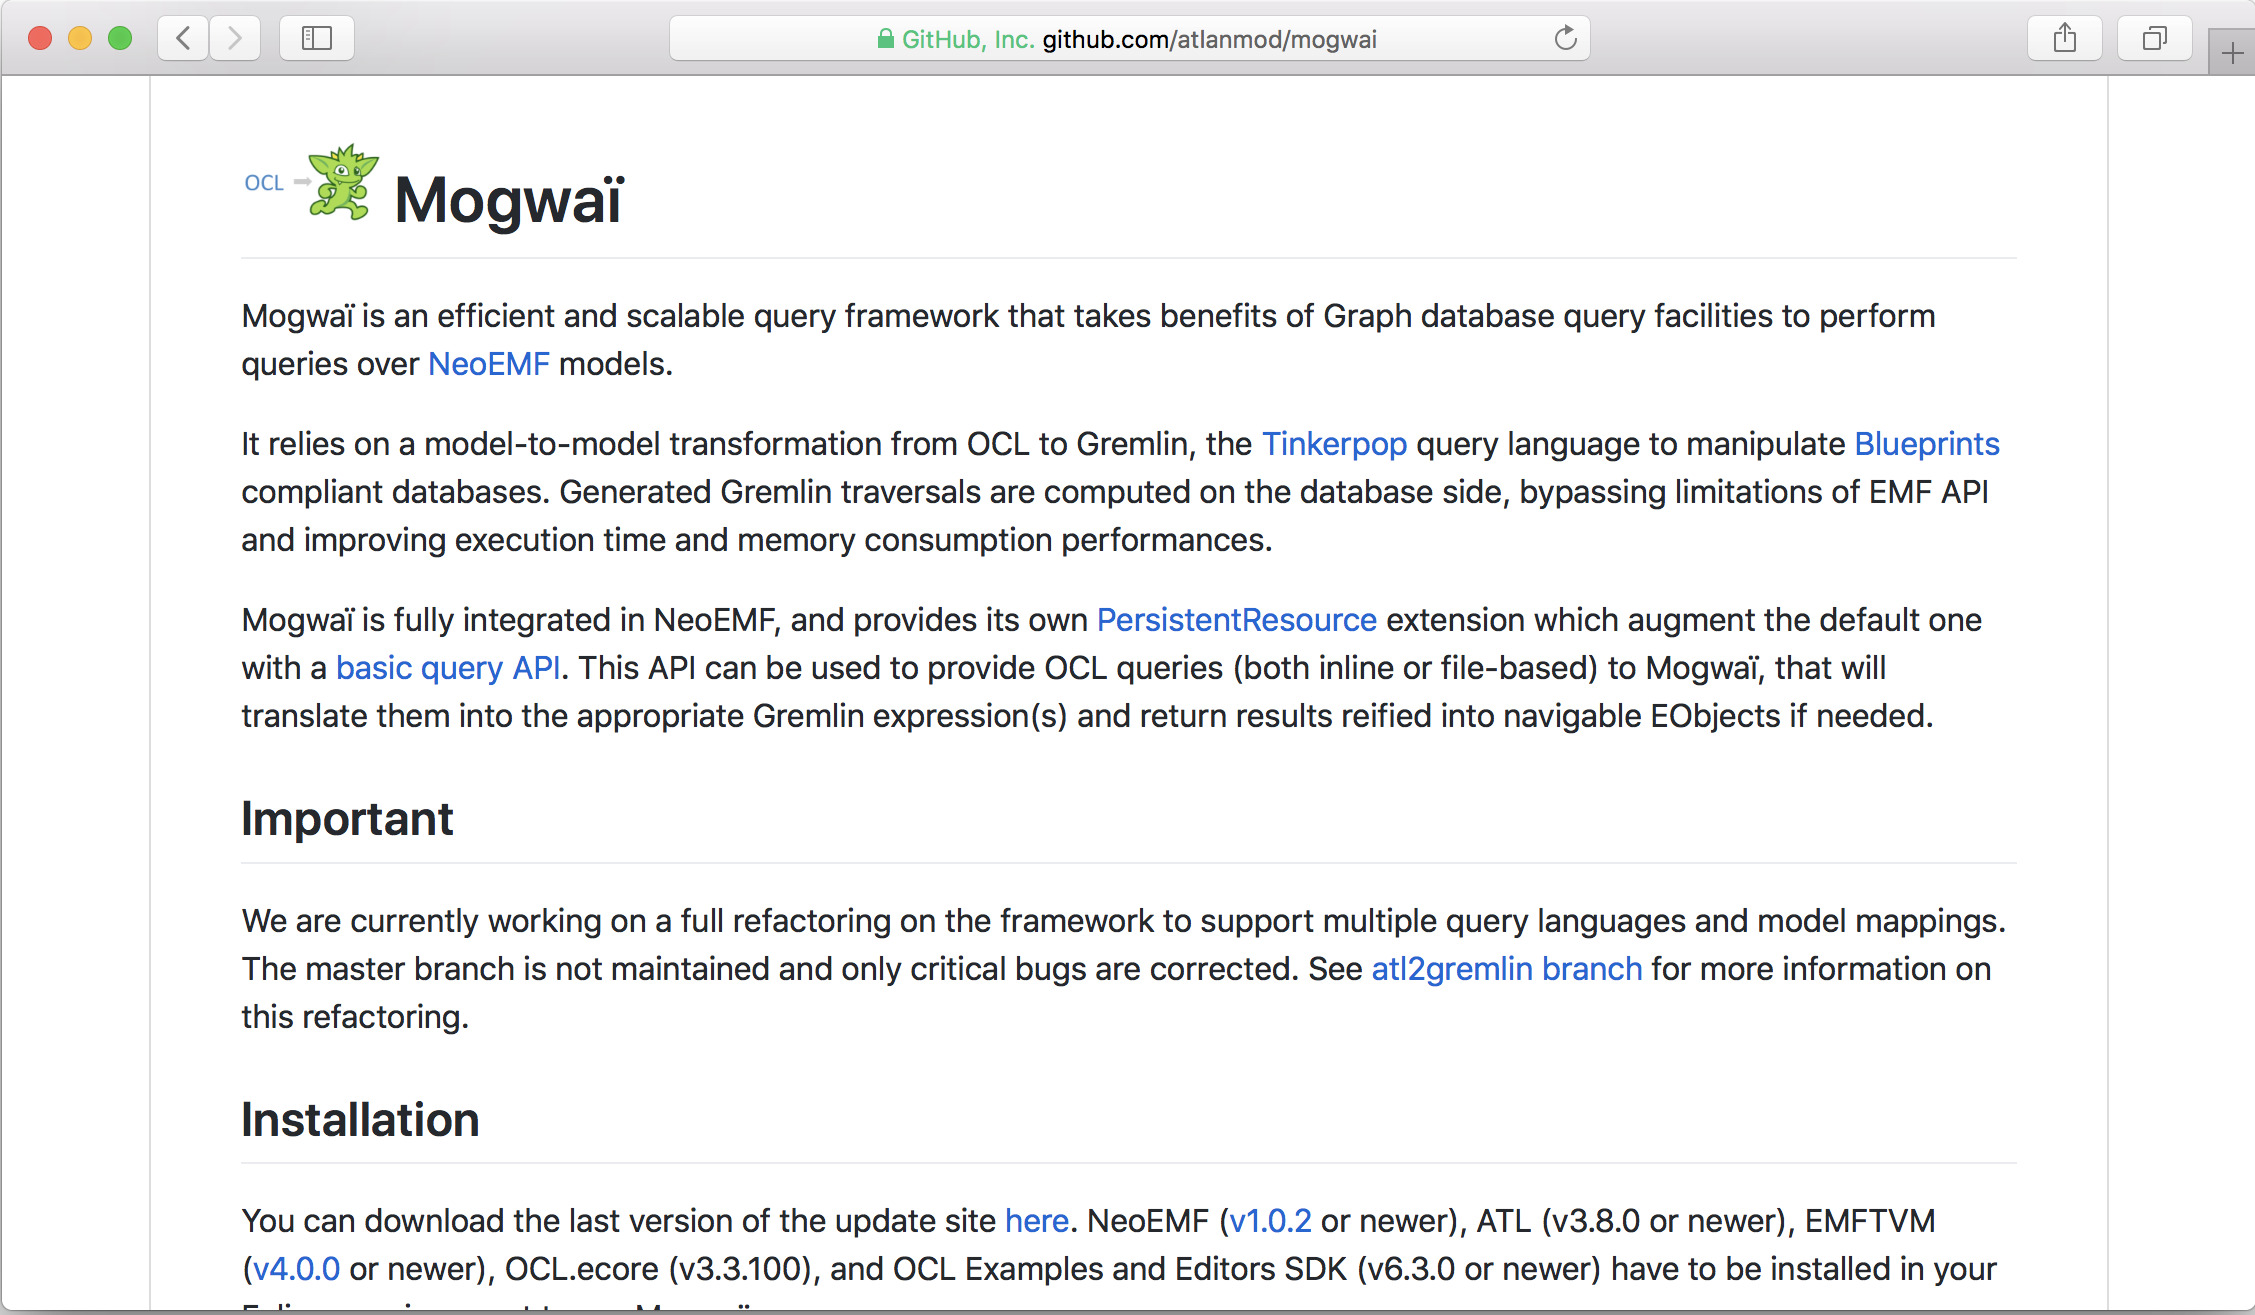
\includegraphics[width=\textwidth]{mogwai-github.png}
  \end{center}
	
  \begin{itemize}
  \item \url{https://github.com/atlanmod/mogwai}
  \item Open source project under the Eclipse Public License 2.0
  \end{itemize}
\end{frame}

\begin{frame}[fragile]\frametitle{Mogwa\"i: load a Mogwa\"i resource}
\begin{enumerate}
	\item Register the BlueprintsPersistenceBackendFactory.
	\item Create a ResourceSet and register the PersistentResourceFactory
	\item Create a new MogwaiURI to locate a file-based resource.
	\item Create and cast the resource.
	\item Use the Mogwa\"i API
	\end{enumerate}
	
  \begin{java}
PersistenceBackendFactoryRegistry.register(
	MogwaiURI.MOGWAI_SCHEME, BlueprintsPersistenceBackendFactory.getInstance());
		
ResourceSet resourceSet = new ResourceSetImpl();
resourceSet.getResourceFactoryRegistry().getProtocolToFactoryMap()
	.put(MogwaiURI.MOGWAI_SCHEME, MogwaiResourceFactory.getInstance());
		
URI uri = MogwaiURI.createMogwaiURI(new File("<db_path>"));

MogwaiResource resource = (MogwaiResource) resourceSet.createResource(uri);
resource.load(Collections.emptyMap());

// Use EMF Resource with enhanced querying API
resource.query([...]);  
  \end{java}
\end{frame}

\begin{frame}[fragile]\frametitle{Mogwa\"i: load and execute an OCL query}
\begin{enumerate}
\item Create a MogwaiQuery
\item Query the resource and get a QueryResult
\item Retrieve the database results, execution time, executed query \ldots
\end{enumerate}
\begin{java}
MogwaiQuery query = OCLQueryBuilder.newBuilder()
	.fromURI(URI.createURI("ocl/singletonMethods.ocl"))
	.build();
	
QueryResult result = resource.query(MogwaiQuery);
result.isSingleResult(); // returns only one element?
result.resultSize(); // number of results
result.getExecutedQuery(); // get the executed database query
result.getComputationTime(); // time to compute the query
result.getResults(); // Collection<Object> of database results
\end{java}
\end{frame}

\begin{frame}[fragile]\frametitle{Mogwa\"i: manipulate query results}
\begin{enumerate}
\item Get a NeoEMFQueryResult
\item Reify the results (if possible\footnote{Primitive types cannot be reified})
\item Navigate your model elements using the standard EMF API
\end{enumerate}
\begin{java}
MogwaiQuery query = OCLQueryBuilder.newBuilder()
	.fromURI(URI.createURI("ocl/singletonMethods.ocl"))
	.build();
	
NeoEMFQueryResult result = resource.query(MogwaiQuery);
if(result.isReifiable()) {
	List<EObject> eObjects = result.reifyResults();
	for(EObject e : eObjects) {
		System.out.println(((MethodDeclaration)e).getName());
	}
}
\end{java}
\end{frame}

\begin{frame}[c]\frametitle{Mogwa\"i: new features}
\begin{itemize}
	\item ModelDatastore abstraction
		\begin{itemize}
		\item Support for different data stores
		\item Easily extensible
		\item Generic queries
		\end{itemize}
	\item Prototype support for model transformations (Gremlin-ATL~\cite{daniel2017gremlin})
	\item Data migration operations
	\item Large model validation (presenting this work at 15:00 at OCL'18)
\end{itemize}

\end{frame}



\begin{frame}[c]\frametitle{NeoEMF \& Mogwa\"i: summing up}
	\begin{block}{NeoEMF}
	  \begin{itemize}
		\item Select the NoSQL database adapted to a modeling scenario
		\item Transparent EMF integration
		\item On-demand loading
	  \end{itemize}
	\end{block}

  \begin{block}{Mogwa\"i}
		\begin{itemize}
		\item Benefit from the capabilities of NeoEMF/Graph backend
		\item Translates OCL queries into Gremlin traversals
		\item Bypasses low-level modeling APIs
	  \end{itemize}
  \end{block}
\end{frame}

\pgfset{/metropolis/inner/sectionpage/.cd, none}
\section{Wrap-up}

\begin{frame}[allowframebreaks]{References}
  \bibliography{../bibliography}
  \bibliographystyle{alpha}
\end{frame}

\end{document}
